\documentclass[a4paper,11pt,bibliography=totoc,listof=totoc,headinclude=true,cleardoublepage=empty,oneside]{scrartcl}
% Option "oneside" für einseitigen Druck. Weglassen, falls die Arbeit doppelseitig gedruckt wird

\usepackage[english,ngerman]{babel}
\usepackage[utf8]{inputenc}
%\usepackage{fullpage}
\usepackage{ifthen}
\usepackage{color}
\usepackage{amsmath,amsthm,amssymb,amsfonts}
\usepackage{graphicx}
\usepackage{psfrag}
\usepackage{float}
\usepackage{blindtext}
\usepackage{listings}
\usepackage{lineno}
\usepackage{tabularx}
\usepackage[linesnumbered,algoruled,boxed,lined]{algorithm2e}

% links in pdf
\usepackage[unicode,colorlinks=true,pagebackref=false]{hyperref}

% Zum Druck verwende schwarze Links!
%\usepackage[unicode,colorlinks=true,linkcolor=black,citecolor=black,urlcolor=black,pagebackref=false]{hyperref} 
	% colorlinks=false umrahmt Links statt einzufaerben, 


% document style
\KOMAoptions{footinclude=false} % Fusszeile wird nicht zu Satzspiegel gezaehlt
\KOMAoptions{headsepline=true} % Trennlinie zwischen Kopfzeile und Text
\KOMAoptions{DIV=12} % beeinflusst Satzspiegel
%\KOMAoptions{BCOR=8mm} % Bindekorrektur
\pagestyle{headings} % mit Kopfzeilen

\recalctypearea % berechne Satzspiegel neu

\definecolor{change}{rgb}{0,.55,.55}

\def\revision#1{{\color{red}#1}}


\setlength{\parindent}{0pt}
\setlength{\parskip}{5pt}

%Belegung einzelner Buchstaben
\newcommand{\A}{\mathcal{A}}
\newcommand{\B}{\mathcal{B}}
%\newcommand{\C}{\mathbb{C}}
\newcommand{\E}{\mathcal{E}}
\newcommand{\F}{\mathcal{F}}
\newcommand{\K}{\mathbb{K}}
\newcommand{\N}{\mathbb{N}}
\newcommand{\OO}{\mathcal{O}}
\newcommand{\Q}{\mathbb{Q}}
\newcommand{\R}{\mathbb{R}}
\newcommand{\T}{\mathsf{T}}


%sonstiges zeug
\renewcommand{\subset}{\subseteq}
\renewcommand{\supset}{\supseteq}
\renewcommand{\epsilon}{\varepsilon}

%markos
\newcommand{\diff}[2]{\frac{\partial #1}{\partial #2}}
\newcommand{\secdiff}[2]{\frac{\partial^2 #1}{\partial^2 #2}}
\newcommand{\diffdiff}[3]{\frac{\partial^2 #1}{\partial #2 \partial #3}}
\newcommand{\norm}[2]{\left\| #1 \right\|_{#2}}

%CODE LISTINGS
\usepackage{xcolor}
\definecolor{mygreen}{rgb}{0,0.5,0}
\definecolor{mygray}{rgb}{0.5,0.5,0.5}
\definecolor{mymauve}{rgb}{0.58,0,0.82}
\usepackage{listings} 
\lstset{ %
	backgroundcolor=\color{white},   % choose the background color; you must add \usepackage{color} or \usepackage{xcolor}; should come as last argument
	basicstyle=\normalfont\ttfamily,        % the size of the fonts that are used for the code
	breakatwhitespace=false,         % sets if automatic breaks should only happen at whitespace
	breaklines=true,                 % sets automatic line breaking
	captionpos=b,                    % sets the caption-position to bottom
	commentstyle=\color{mygreen},    % comment style
	deletekeywords={...},            % if you want to delete keywords from the given language
	escapeinside={\%*}{*)},          % if you want to add LaTeX within your code
	extendedchars=true,              % lets you use non-ASCII characters; for 8-bits encodings only, does not work with UTF-8
	frame=single,	                   % adds a frame around the code
	keepspaces=true,                 % keeps spaces in text, useful for keeping indentation of code (possibly needs columns=flexible)
	keywordstyle=\color{blue},       % keyword style
	language=Matlab,                 % the language of the code
	morekeywords={*,...},            % if you want to add more keywords to the set
	numbers=left,                    % where to put the line-numbers; possible values are (none, left, right)
	numbersep=5pt,                   % how far the line-numbers are from the code
	numberstyle=\footnotesize\color{mygray}\ttfamily, % the style that is used for the line-numbers
	rulecolor=\color{black},         % if not set, the frame-color may be changed on line-breaks within not-black text (e.g. comments (green here))
	showspaces=false,                % show spaces everywhere adding particular underscores; it overrides 'showstringspaces'
	showstringspaces=false,          % underline spaces within strings only
	showtabs=false,                  % show tabs within strings adding particular underscores
	stepnumber=1,                    % the step between two line-numbers. If it's 1, each line will be numbered
	stringstyle=\color{mymauve},     % string literal style
	tabsize=2,	                   % sets default tabsize to 2 spaces
	title=\lstname                   % show the filename of files included with \lstinputlisting; also try caption instead of title
}
\newcounter{satz}
\setcounter{satz}{1}

\begin{document}

% TITELSEITE 


\pagenumbering{Alph}
\selectlanguage{ngerman}

\begin{titlepage}
  %\vspace*{-2cm}
  \begin{center}
    
\includegraphics[width=0.45\textwidth]{TULogo.eps}
    \vskip 1cm%
    {\LARGE N~\Large U~M~E~R~I~K~P~R~O~J~E~K~T}
    \vskip 8mm
    {\huge\bfseries\color{change}Titel \\[1ex] ggf.\ mehrzeilig}
    \vskip 1cm
    \large 
    ausgef\"uhrt am    
    \vskip 0.75cm
    {\Large Institut f\"ur\\[1ex] Analysis und Scientific Computing}\\[1ex]
    {\Large TU Wien}
    \vskip0.75cm
    unter der Anleitung von
    \vskip0.75cm
    {\Large\bfseries Prof. Dr. Lothar Nannen}\\[1ex]
    \vskip 0.5cm
    durch
    \vskip 0.5cm
    {\Large\bfseries Lukas Moser }\\[1ex]
    Matrikelnummer: {1607333}\\[1ex]
    {\Large\bfseries Stefan Schrott}\\[1ex]
    Matrikelnummer: {1607388}\\[1ex]
   
  \end{center}
  
  \vfill
  
  \small
  Wien, am \today
  \vspace*{-15mm}
\end{titlepage}

\cleardoublepage

%%%%%%%%%%%%%%%%%%%%%%%%%%%%%%%%%%%%%%%%%%%%%%%%%%%%%%%%%%%%%%%%%%%%%%%%%%%%%%%%%%%%%%%%%%%%%%%%%%%%%%%%%%%%%%
% INHALTSVERZEICHNIS [OBLIGATORISCH]
%%%%%%%%%%%%%%%%%%%%%%%%%%%%%%%%%%%%%%%%%%%%%%%%%%%%%%%%%%%%%%%%%%%%%%%%%%%%%%%%%%%%%%%%%%%%%%%%%%%%%%%%%%%%%%

\pagenumbering{roman}
\selectlanguage{ngerman} 

\tableofcontents

\cleardoublepage
\pagenumbering{arabic} 


\section{Grundlagen}
Die Grundlage für die folgenden Überlegung ist der Hauptsatz über implizite Funktionen im Spezialfall von Funktionen $F: A \times B \to \R$, wobei $A$ und $B$ der Einfachheit halber offene Intervalle seien.

\textbf{Satz \thesatz\refstepcounter{satz}:} Seien $a<b$ sowie $c<d \in \R$ und $F : (a,b) \times (c,d) \to \R$ stetig differenzierbar. Seien $x_0 \in (a,b)$ und $y_0 \in (c,d)$, sodass $F(x_0,y_0)=0$ und $\diff{F}{y}(x_0,y_0) \neq 0$. 

Dann existieren $a_0,b_0 \in \R$ mit $a<a_0<x_0<b_0<b$ und eine stetig differenzierbare Funktion $f : (a_0,b_0) \to \R$ mit $f(x_0)=y_0$, sodass 
\[
\forall x \in (a_0,b_0) : F(x,f(x))=0
\]
und
\begin{align}\label{eq:fstrich}
\forall x \in (a_0,b_0) :  f'(x) = - \frac{\diff{F}{x}(x,f(x))}{\diff{F}{y}(x,f(x))}.
\end{align}

\textbf{Beweis:} Unter den gegebenen Voraussetzungen ist der Hauptsatz über implizite Funktionen anwendbar und liefert Umgebungen $U$ von $x_0$ und $V$ von $y_0$ und eine Funktion $f: U \to V$ mit den geforderten Eigenschaften. Da $x_0$ ein innere Punkt von $U$ ist, enthält $U$ ein Intervall $(a_0,b_0)$ mit den geforderten Eigenschaften.

Die Umgebung $V \subset \R$ in der Zielmenge von $f$ kann durch ganz $\R$ ersetzt werden, da wir nur behauptet haben, dass $y=f(x)$ eine Lösung von $F(x,\:\cdot \:)=0$ ist, allerdings nicht dass diese eindeutig ist. \hfill
$\blacksquare$

\textbf{Satz \thesatz\refstepcounter{satz}:} Sei unter den Vorraussetzungen des vorherigen Satz $F$ zwei mal stetig differenzierbar.
Dann ist $f \in C^2((a_0,b_0))$ mit $f''(x) = $
\[
\frac{ \!-\secdiff{F}{x}(x,f(x)) \left( \diff{F}{y}(x,f(x)) \right)^2 \!\!\! +\! 2 \diffdiff{F}{x}{y}(x,f(x))\diff{F}{x}(x,f(x))\diff{F}{y}(x,f(x)) \!-\! \secdiff{F}{y}(x,f(x)) \left( \diff{F}{x}(x,f(x)) \right)^2  }{ \left(\diff{F}{y}(x,f(x))\right)^3 }.
\]
Außerdem gilt:
\[
\forall x \in (a_0,b_0) \exists \xi \in (x_0,x)\cup (x,x_0) : f(x) = y_0 + \frac{\diff{F}{x}(x_0,y_0)}{\diff{F}{y}(x_0,y_0)}(x-x_0) + \frac{f''(\xi)}{2}(x-x_0)^2.
\]
\textbf{Beweis:} Aus $F \in C^2$ folgt mit der Kettenregel und Einsetzen der Darstellung \eqref{eq:fstrich} für $f'$:
\begin{align*}
\frac{d}{dx}\left( \diff{F}{x}(x,f(x))  \right) &= \left( \secdiff{F}{x}(x,f(x)) , \diffdiff{F}{x}{y}(x,f(x))  \right) \cdot \binom{1}{f'(x)} \\
&= \secdiff{F}{x}(x,f(x)) - \diffdiff{F}{x}{y}(x,f(x)) \frac{\diff{F}{x}(x,f(x))}{\diff{F}{y}(x,f(x))}.
\end{align*}
Für $\frac{d}{dx}\left( \diff{F}{y}(x,f(x))  \right)$ erhält man analog eine ähnliche Darstellung. Damit kann man den Ausdruck \eqref{eq:fstrich} mithilfe der Quotientenregel differenzieren und erhält durch Erweitern mit $\diff{F}{y}(x,f(x))$ obige Darstellung für $f''$.

Die zweite Aussage folgt aus dem Satz von Taylor und der Tatsache, dass $f''$ als Komposition stetiger Funktionen stetig ist. \hfill $\blacksquare$

\section{Aufgabe a}
Das Ziel dieser Aufgabenstellung ist es den Graphen, der durch die Nullstellenmenge einer Funktion, numerisch anzunähern. Im ersten Schritt wollen wir dazu einem Gitter $x_j = x_0 + j*h, j \in \left\lbrace1...n\right\rbrace $ entlang x folgen. 
Dazu soll die Funktion $F$ auf der gesamten betrachteten Menge die Bedingungen des Hauptsatzes über implizite Funktionen erfüllen und $F(x_0,y_0)=0$ sein. Damit wissen wir, dass $\forall j \in \left\lbrace1...n\right\rbrace: F(x_j,f(x_j)=0)$ gilt. Um $y_n = f(x_n)$ zu berechnen betrachte man mittels Mittelwertsatz
\[
f(x_{n+1})=f(x_n)+f'(x_n)*h+r_n, \left|r_n\right|\leq \sup\limits_{a,b \in \left[x_n,x_{n+1}\right]}\left|{f'(a)-f'(b)}\right|*h.
\]
Demnach ist für hinreichend kleine Schrittweite das Restglied $r_n$ klein genug, so dass die Nullstelle für $F(x_{n+1},.)$ und somit $f(x_{n+1})$ mittels Newtonverfahren gefunden werden kann.
\subsection{Implementierung}
\begin{algorithm}
	\label{alg:A_const_h}
	\SetKwInOut{Input}{Input}
	\SetKwInOut{Output}{Output}
	\Input{$F$...Funktion\\
		$(x_0,y_0)$...Startpunkt\\
		$h$...Schrittweite\\
		$n$...Schrittzahl}
	\Output{$(x_j,y_j)_{j\in \left[1,n\right] }$}
	\For {i = 1 to n} 
	{
		$x_i = x_{i-1}+h$\\
		$df = -\frac{\diff{F}{x}(x_{i-1},y_{i-1})}{\diff{F}{y}(x_{i-1},y_{i-1})}$\\
		$\tilde y_i = y_{i-1}+h*df$\\
		$G(a) = F(x_i,a)$\\
		$y_i$ = Newton($G$, $\tilde y_i$)
	}
	\caption{Kurve A}
\end{algorithm}
Die Implementierung ist eine einfache Umsetzung von Algorithmus \ref{alg:A_const_h}.
Fehlschlagen können dabei folgende 3 Punkte:
\begin{itemize}
	\item $\diff{F}{y}(x_{i-1},y_{i-1})$ kann 0 sein. Das wurde im Vorhinein ausgeschlossen.
	\item Das Newton verfahren kann keine Nullstelle finden bzw findet eine falsche Nullstelle. Das kann behoben werden indem man die Schrittweite reduziert.
\end{itemize}
\subsection{Tests}
Wie zu erwarten war, ist die Darstellung an Stellen in denen $f'(x)$ groß wird sehr ungenau, vor allem bei großen Schrittweiten. Siehe Abbildung \ref{fig:Halbkreis_a}.
\begin{figure}[h]
\centering
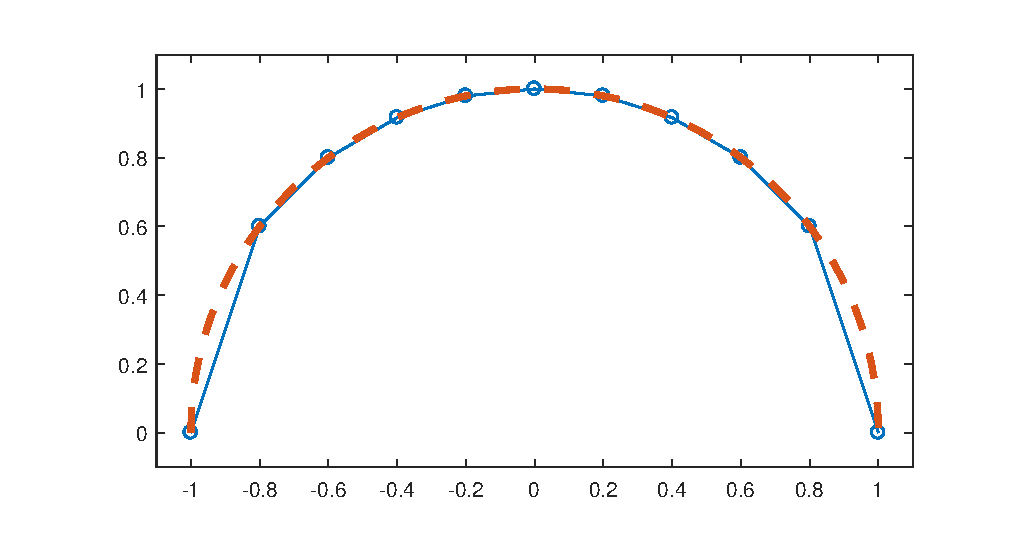
\includegraphics[width=0.85\linewidth]{plots/A/Halbkreis.eps}
\caption{Plot zweier Halbkreise mit Schrittweiten $10^{-3}$ und $0.2$}
\label{fig:Halbkreis_a}
\end{figure}
Wenn die darzustellende Funktion für ein $x$ mehr als ein $y$ hat so dass $F(x,y)=0$ so kann es passieren, dass das Newtonverfahren gegen die falsche Nullstelle konvergiert. Ob die gefundene Nullstelle die Korrekte ist oder nicht, ist nur unter großem Aufwand feststellbar. Als Beispiel für so ein Funktion und zur Untersuchung des Verhaltens des Algorithmus verwenden wir
\begin{align*}
G(x,y) = \sin(10*\pi*(sin(x)-y))
\end{align*}
mit Nullstellen
\begin{align*}
\left\lbrace (x,y)\in\mathbb{R}: G(x,y)=0 \right\rbrace = \left\lbrace (z, \sin(z)+n*0.1): z \in \mathbb{R}, n \in \mathbb{N} \right\rbrace
\end{align*}
Wie Abbildung \ref{fig:vieleSinuse_schrittweiten_a} zu entnehmen ist beginnt der Algorithmus ab einer Schrittweite $\geq \frac{\pi}{8}$ falsche Nullstellen zu finden.
\begin{figure}[h]
\centering
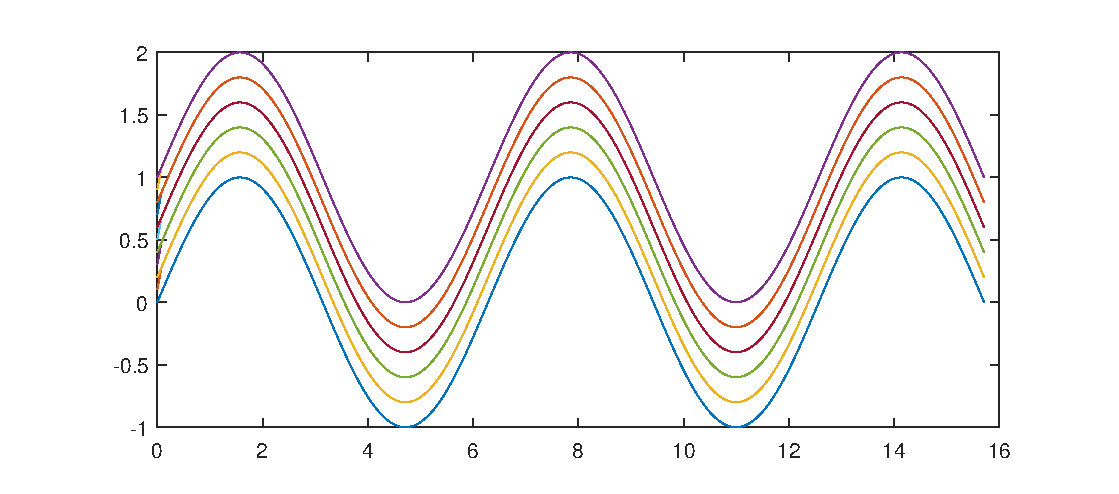
\includegraphics[width=0.85\linewidth]{plots/A/vieleSinuse.eps}
\caption{Illustration der Nullstellenmenge von $G$.}
\label{fig:vieleSinuse_a}
\end{figure}
\begin{figure}[h]
\centering
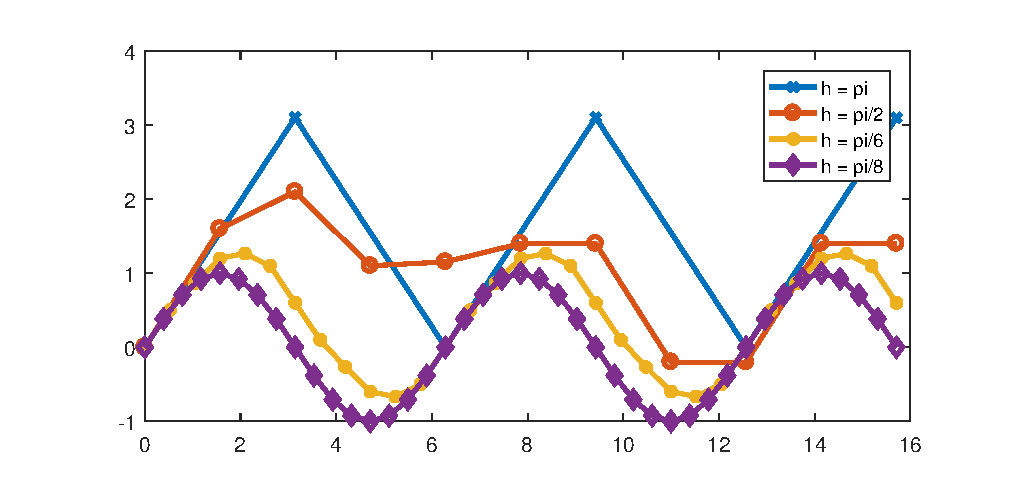
\includegraphics[width=0.85\linewidth]{plots/A/vieleSinuse_Schrittweiten.eps}
\caption{$G$, $x_0 = y_0 = 0$ dargestellt mit verschiedenen Schrittweiten.}
\label{fig:vieleSinuse_schrittweiten_a}
\end{figure}


\section{Aufgabe b}
Die Voraussetzung des Satzes über implizite Funktionen, dass die Ableitung nach $y$ nicht $0$ werden darf ist sehr restriktiv, da so nicht einmal ein Kreis gezeichnet werden kann. Es ist möglich diese Voraussetzung abzuschwächen indem man fordert, dass in den Nullstellen entweder die Ableitung nach $x$ oder $y$ ungleich $0$ sein müssen. Dadurch kann die Nullstellenmenge der Funktion durch offene Mengen überdeckt werden für die jeweils $F(x,f(x))=0$ oder $F(g(y),y)=0$ gilt.
\subsection{Implementierung Version 1}
%also mit 90 Drehungen
Die einfachste Variante auf Aufgabe a basierend Aufgabe b zu implementieren ist rekursiv den Algorithmus aufzurufen, wenn die Betragsmäßige Ableitung in eine Richtung größer wird als die andere. Wichtig dabei ist auf folgendes zu achten, dass der Wechsel Richtung früh genug erfolgt, damit der Bereich mit Nullstellen nicht in eine Richtung verlassen wird und dass der Richtungswechsel mit dem korrekten Vorzeichen passiert. 
\begin{algorithm}[h]
	\label{alg:B_V1}
	\SetKwInOut{Input}{Input}
	\SetKwInOut{Output}{Output}
	\Input{$F$...Funktion\\
		$(x_0,y_0)$...Startpunkt\\
		$h$...Schrittweite\\
		$n$...Schrittzahl}
	\Output{$(x_j,y_j)_{j\in \left[1,n\right] }$}
	\For {i = 1 to n} 
	{
		dx = $\diff{F}{x}(x_{i-1},y_{i-1})$\\
		dy = $\diff{F}{y}(x_{i-1},y_{i-1})$\\
		\eIf{abs(dy)$<$abs(dx)}
		{
			$G(a,b)$ = $F(b,a)$\\
			dir = 1
			\uIf{abs(dy) $>$ TOL}
			{dir = sgn(dy)}
			\ElseIf{i $>$ 1}
			{dir = sgn($y_{i-1}$-$y_{i-2}$)}
			$(x_k,y_k)_{i..n}$ = KurveB1($G$,$(y_{i-1},x_{i-1})$,abs($h$)*dir, n-i)\\
			return
		}
		{
			$x_i = x_{i-1}+h$\\
			$\tilde y_i = y_{i-1}+h*df$\\
			$G(a) = F(x_i,a)$\\
			$y_i$ = Newton($G$, $\tilde y_i$)
		}
	}
	\caption{Kurve B1}
\end{algorithm}
Nachteile dieser Implementierung liegen darin, dass es aufwändig ist vorherzusagen wie lang die Kurve wird. In Algorithmus \ref{alg:A_const_h} läuft die Kurve von $\left\lbrace x_0\right\rbrace \times\mathbb{R}$ bis $\left\lbrace x_0+h*n\right\rbrace \times\mathbb{R}$. Das bedeutet für $m\in \mathbb{N}$, dass man einen Viertelkreis mit $n=m$ und $h=\frac{1}{m}$ zeichnen kann. Mit Algorithmus \ref{alg:B_V1} benötigt man dafür $n=\lceil m*\sqrt{2}\rceil$ und $h=\frac{1}{m}$, da der Richtungswechsel bei $x_i\approx \sin(\frac{\pi}{4})$ stattfindet.
\subsection{Implementierung Version 2}
%das mit beliebiger Richtung
Um die Probleme mit Version 1 zu beheben, vor allem, wenn beide Ableitungen sehr klein sind ist es möglich nicht nur entlang der Richtungen der kanonischen Basisvektoren zu arbeiten. Stattdessen ist es möglich eine Orthonormalbasis mit Basistransformation $t_\phi$ zu finden, so dass für $G(x,y) = F(t_\phi(x,y))$ die Ableitung der impliziten Funktion $g'(x)=0$ ist.
Dies ist einfach zu verifizieren, da
\begin{align}
	t_\phi(x,y) = (x*cos(\phi)-y*sin(\phi), x*sin(\phi)+y*cos(\phi))\\
	g'(x) = -\frac{\diff{G}{x}(x,y)}{\diff{G}{y}(x,y)}\\
	\diff{G}{x}(x,y) = \diff{F}{x}(t_\phi(x,y))*cos(\phi)+\diff{F}{y}(t_\phi(x,y))*sin(\phi)=c(x,y)*sin(\phi + \psi(x,y))\\
	\diff{G}{y}(x,y)=c(x,y)*cos(\phi + \psi(x,y))
\end{align}
Dadurch ist nun $h*n$ annähernd die Kurvenlänge und die Genauigkeit des Prediktorschritts ist unabhängig von der ersten Ableitung von $F$.
Da die $\diff{G}{x}(x,y)$ für $\phi$ und $\phi+\pi$ gleich ist und damit keine eindeutige Richtung vorgegeben ist, müssen andere Punkte dafür herangezogen werden. Mögliche Ansätze sind u.a. positives Skalarprodukt zwischen aktuellem und letzten Richtungsvektor oder minimale Differenz zwischen aktuellem und letzten $\phi$.

\begin{algorithm}[h]
	\label{alg:B_V2}
	\SetKwInOut{Input}{Input}
	\SetKwInOut{Output}{Output}
	\Input{$F$...Funktion\\
		$(x_0,y_0)$...Startpunkt\\
		$h$...Schrittweite\\
		$n$...Schrittzahl}
	\Output{$(x_j,y_j)_{j\in \left[1,n\right] }$}
	\For {i = 1 to n} 
	{
		dx = $\diff{F}{x}(x_{i-1},y_{i-1})$\\
		dy = $\diff{F}{y}(x_{i-1},y_{i-1})$\\
		\eIf{dx == 0}
		{
			$x_i = x_{i-1}+h$\\
			$\tilde y_i = y_{i-1}$\\
			$G(a) = F(x_i,a)$\\
			$y_i$ = Newton($G$, $\tilde y_i$)	
		}
		{
			$\psi$ = atan(dy/dx)			//Richtung maximaler Ableitung\\
			$\phi$ = $\psi-\frac{\pi}{2}$	//Richtung minimaler Ableitung\\
			$\phi$ = correctPhi($\phi$)\\
			$\psi$ = $\phi+\frac{\pi}{2}$	//psi mitkorrigieren\\
			$\tilde x_i = x_{i-1}+h*cos(\phi)$\\
			$\tilde y_i = y_{i-1}+h*sin(\phi)$\\
			$G(a)$ = $F(\tilde x_i+a*cos(\psi),\tilde y_i+a*sin(\psi))$\\
			s = Newton($G$, 0)\\
			$x_i = \tilde x_{i}+s*cos(\psi)$\\
			$y_i = \tilde y_{i}+s*sin(\psi)$\\
		}
	}
	\caption{Kurve B2}
\end{algorithm}
\subsection{Tests}


\section{Implementierung von adaptiver Schrittweite}
Das Ziel von adaptiver Schrittweite ist es im Idealfall, dass der Abstand des Polygonzuges durch die Punkte $(x_i,y_i)$ zur Nullstellenmenge kleiner ist als eine vorgegebene Konstante und dafür möglichst wenige Punkte bzw. möglichst wenig Rechenzeit benötigt werden.

Für den die adaptive Schrittweite ergeben sich zwei Problemstellungen:
\begin{enumerate}
	\item Die Datenpunkte $(x_i,y_i)$ sollen möglichst sein.
	\item Der Polygonzug soll die Nullstellenmenge möglichst gut approximieren.
\end{enumerate}

Die erste Problemstellung ist recht einfach zu lösen: Durch das Newton-Verfahren im Korrektor-Schritt ist $(x_i,y_i)$ extrem an einer Nullstelle -- die dabei bleibende geringe Abweichung wird auch nicht Schrittweite des Prediktors beeinflusst. Das einzige was hier zu tun ist, ist also die Schrittweite zu verkleinern, falls das Newton-Verfahren nicht konvergiert. 

Die zweite Problemstellung ist die wesentlich interessanter, die im folgenden zu lösen versucht wird. Der Einfachheit halber werden mögliche Strategien für adaptive Schrittweite zuerst an der Implementierung aus Aufgabe a getestet, da das Koordinatensystem dort noch fest ist. Dann werden sie, falls möglich und sinnvoll, auf den allgemeinen Fall ausgeweitet.

Wir gehen bei den Überlegungen dazu überdies davon aus, dass die Datenpunkte selbst korrekt sind bzw. dass wir deren Fehler vernachlässigen können.
\subsection{Mögliche Strategien für Aufgabe a}\label{chap:5.1}
Wir nehmen nun an, dass es auf $(a,b)$ eine Funktion $f$ gibt, sodass $F(x,f(x))=0$ für alle $x \in (a,b)$. 

Es ergeben sich folgende mögliche Strategien:
\begin{enumerate}
	\item Die Krümmung von $f$  im letzten Punkt explizit berechnen
	\item Versuchen, die Krümmung von $f$ aus den letzten Punkten zu schätzen 
	\item Die Differenz von Prediktor und Korrektor betrachten
\end{enumerate}


\subsubsection{Abschätzung der Schrittweite anhand der Krümmung von $f$}\label{chap:5.1.1}

 Zusätzlich dazu nehmen wir an, dass $F \in C^2((a,b))$, was nach Satz ... eine hinreichende Bedingung für $f \in C^2((a,b))$ ist. Außerdem liefert der Satz dann eine explizite Darstellung von $f''$.  

Sei $x_0 \in (a,b)$ ein Startwert und $c>0$ eine vorgegebene Toleranz. Das Ziel ist es nun, ein (möglichst großes) $h \in (0,h_{max})$ zu finden, sodass die Gerade zwischen $(x_0,f(x_0))$ und $(x_0+h,f(x_0+h))$ maximal um $c$ von $f$ abweicht. Hat man so ein $h$ gefunden, kann man $x_1 := x_0+h$ setzen und von dort aus fortfahren, um insgesamt einen Polygonzug zu erhalten, für den diese Abschätzung gilt. 

Bei einen einzelnen Iterationsschritt handelt es sich dabei um eine lineare Interpolationsaufgabe, da wir nach dem Korrektorschritt davon ausgehen können, dass $f(x_0)$ und $f(x_0+h)$ nahezu korrekt ist. Es geht hier also um die Frage, wie sich $f$ zwischen diesen Punkten verhält, insbesondere wie sehr es von einer Geraden durch die Punkte $(x_0,f(x_0))$ und $(x_0+h,f(x_0+h))$ abweicht.

 Die Gleichung der Interpolationsgeraden $g_h$ ist gegeben durch (vgl Skriptum Bsp 3.17):
\[
g_h (x) = \frac{f(x_0)(x_0+h-x) + f(x_0+h)(x-x_0)}{h},
\]
wobei dann folgende Abschätzung gilt:
\[
\sup_{x \in [x_0,x_0+h]} |f(x)-g_h(x)|  \le \frac{h^2}{8} \sup_{x \in [x_0,x_0+h]} |f''(x)| \le \frac{h^2}{8} \sup_{x \in [x_0,x_0+h_{max}]} |f''(x)|.
\]
Es gilt:
\[
c = \frac{h^2}{8} \sup_{x \in [x_0,x_0+h_0]} |f''(x)| \quad \iff \quad h = \sqrt{ \frac{8c}{\sup_{x \in [x_0,x_0+h_{max}]} |f''(x)|}}.
\]

Daher gilt für $h \in (0,h_{max})$:
\begin{align}\label{eq:absch_h}
\quad h \le \sqrt{ \frac{8c}{\sup_{x \in [x_0,x_0+h_{max}]} |f''(x)|}} \quad \implies \quad \sup_{x \in [x_0,x_0+h]} |f(x)-g_h(x)| \le c.
\end{align}

Da das numerische Berechnen des Supremums nicht möglich ist, kann man an dieser Stelle nicht mehr so weiterarbeiten, dass obige Abschätzungen garantiert werden. In einem ersten Schritt kann man heuristisch
\[
h := \sqrt{\frac{8c}{|f''(x_0)| +\frac{8c}{h_{max}^2} }} \in (0,h_{max})
\]
wählen. Dann sind zwar keine der obigen Abschätzungen garantiert, man hat einen ersten Ansatz für adaptive Schrittweite. Zusätzlich dazu wird bei der Implementierung auch eine Mindestschrittweite vorgegeben, die nicht unterschritten werden darf. 


\subsubsection{Schrittweitensteuerung durch Länge der Korrektorschrittes}\label{chap:5.1.3}
Der Prediktor tut nichts anderes als eine Tangente $t_i(x)$ entlang von $f$ durch den Punkt $(x_i,f(x_i))$ zu legen und anhand dessen einen Punkt $(x_{i+1},\tilde{y}_{i+1})$ zu berechnen, der dann durch einen Korrektorschritt zum Punkt $(x_{i+1},f(x_{i+1}))$ korrigiert wird. Bezeichne $d:= |f(x_{i+1})-\tilde{y}_{i+1}|$ die Länge des Korrektorschrittes. 

Ein Vorteil dieses Verfahrens ist, dass es sehr wenig Aufwand hat und weder $F \in C^2$ gefordert werden muss noch Ableitungen zweiter Ordnung benötigt werden. 

Ein Nachteil ist, dass man erst nach dem Prediktor- und Korrektschritt $d$ erhält und dann "falls $d$ zu groß war", Prediktor- und Korrektschritt wiederholen muss. Das zweite Problem, ist dass vorerst nicht klar, ist aber welcher Schranke für $d$ man den Iterationsschritt wiederholen soll und um wie viel keiner die Schrittweite dann sein soll.

Um die intuitiv vernünftige Tatsache, dass ein großer Korrektorschritt ein Anzeichen dafür ist, dass $f$ nicht gut approximiert wird, auch formal plausibel zu machen und ein Gefühl dafür zu bekommen, welche $d$ ''zu groß'' sind, kann man sich folgendes überlegen:

Wir wissen, dass $(f-t_i)(x_i)=0$, $(f-t_i)'(x_i)=0$ und $(f-t_i)''=f''$. Daraus erhält man mit dem Satz von Taylor im Entwickungspunkt $x_i$:
\[
\exists \xi \in (x_i,x_{i+1}) : (f-t_i)(x_{i+1}) = \frac{f''(\xi)}{2}(x_{i+1}-x_i)^2 = \frac{f''(\xi)}{2}h^2.
\]
Wegen $\frac{f''(\xi)}{2}(x_{i+1}-x_i)^2$ kann man daraus folgern, dass
\[
\exists \xi \in (x_i,x_{i+1}) : h = \sqrt{\frac{2d}{|f''(\xi)|}}.
\]
War nun $d > 4c$ folgt daraus sofort, dass die Ungleichung auf der linken Seite der Implikation in Formel \eqref{eq:absch_h} verletzt ist. Man kann daraus natürlich nicht schließen, dass daher die Abschätzung auf der rechten Seite dieser Implikation verletzt sein muss, aber es macht dennoch plausibel, dass $h$ ungünstig groß gewesen ist. 

Man sieht daraus auch, dass es die Toleranz für $d$ in der Größenordnung von $c$ wählen sollte und der Faktor, um dem man die Schrittweite gegebenenfalls verringert, proportional zu $\sqrt{d/c}$ sein sollte. Bei der Implementierung wird man zusätzlich fordern, dass der Faktor jedenfalls größer 2 sein muss, um nicht mehrmals hintereinander mit sehr ähnlichen Schrittweiten zu arbeiten. Außerdem wird man auch hier eine Mindestschrittweite festlegen.

\subsection{Implementierungen}
Da bei adaptiver Schrittweite für den Nutzer im Vorhinein nicht mehr absehbar ist, wie weit die Nullstellenmenge bei gegebener Schrittanzahl gezeichnet ist, wird nun die Länge des Polygonzuges als Abbruchkriterium verwendet.

Die Funktionen haben also jetzt folgende Form:
\begin{verbatim}
[ x, y, z, steps ] = 
    implicitCurveAdapt( F, dFx, dFy, d2Fxx, d2Fxy, d2Fyy, x0, y0, length,
    maxStepWidth, minStepWidth, c )
\end{verbatim}
Dabei sind die Eingabe-Parameter:
\begin{itemize}
	\item Die ersten sechs sind $F$ bzw deren Ableitungen (werden die Ableitungen 2. Ordnung nicht gebraucht, entfallen sie)
	\item \verb|x0| und \verb|y0| sind die Startwerte
	\item \verb|length| ist die Ziel-Länge des Polygonzuges
	\item \verb|maxStepWidth| und \verb|minStepWidth| geben der Bereich für die Schrittweite an
	\item \verb|c| ist die Konstante $c$ aus Kapitel \ref{chap:5.1}.
\end{itemize}

Die Ausgabe-Daten sind:
\begin{itemize}
	\item \verb|x| und \verb|y| sind die Vektoren der Eckpunkte des Polygonzuges.
	\item \verb|z| dient zur Ausgabe eines der Parameter für die adaptive Schrittweite (zu Testzwecken)
	\item \verb|steps| ist die Anzahl der benötigten Schritte.
\end{itemize}

Es sind folgende Funktionen implementiert worden:
\begin{enumerate}
	\item Adaptive Schrittweite nach Kapitel \ref{chap:5.1.1} sowie Halbierung der Schrittweite, falls das Newton-Verfahren nicht konvergiert,
	%\item Adaptive Schrittweite nach Kapitel \ref{chap:5.1.2} sowie Halbierung der Schrittweite, falls das Newton-Verfahren nicht konvergiert,
	\item Adaptive Schrittweite nach Kapitel \ref{chap:5.1.3} mit Reduktion der Schrittweite um den Faktor $\sqrt{d/c}$, falls $d>c$ sowie Halbierung der Schrittweite, falls das Newton-Verfahren nicht konvergiert,
	\item Eine Kombination der Kriterien aus den beiden vorherigen Kriterien, wobei das zweite erst bei $d>5c$ greift.
\end{enumerate}

Ein Listing des Codes der 4. Version befindet sich im Anhang. 

%vielleicht will man das auch in mit A und mit C aufteilen
\subsection{Tests}
Die Strategien wurden für die Funktion $F(x,y) := \sin(x^2)-y$ getestet. Die Nullstellenmenge von $F$ ist also genau der Graph von $f(x)=\sin(x^2)$. Dabei war Parameter \verb|length| jeweils 200, die Schrittweite durfte zwischen 1 und $10^{-10}$ variieren. Der Parameter \verb|c| wurde so gewählt, dass die verschiedenen Strategie jeweils möglichst gleich viele Schritte benötigten, um die Ergebnisse sinnvoll vergleichen zu können.

In Abbildung \ref{fig:br} sieht man, dass die gemischte Strategie besser ist als ein alleiniges Betrachten der Krümmung im vorherigen Punkt. Beim ersten Schritt ist startet man im Punkt $(0,f(0))$, wo $f''(x) = (\sin(x^2))''= 2\cdot \cos(x^2) - 4\cdot x^2 \cdot \sin(x^2)$ den Wert 2 hat, also im Vergleich zu den Werten von $f''$ klein ist. Daher wird eine zu große Schrittweite verwendet. Bei $x\approx2.521$ hat $f''$ ungefähr den Wert 0.160, was zu einer so großen Schrittweite führt, das ein Teil der Graphen übersprungen wird. Bei der gemischten Strategie war der Korrektorschritt dort aber dann so groß, dass die Schrittweite verkleinert wurde und es zu keinen Problemen kam. Später wird das Verhalten dieses Verfahren besser, weil die Funktionswerte von $f''$ tendenziell größer werden.

In Abbildung \ref{fig:bg} sieht man, dass die gemischte Strategie dem alleinigen Betrachten der Länge des Korrektorschrittes deutlich überlegen ist. Insbesondere wenn die Schwingung von $\sin(x^2)$ schon sehr groß ist, kann es passieren, dass auch bei sehr großer Schrittweite der Korrektorschritt nur sehr klein ist, weil ''zufällig'' fast eine Nullstelle von $F$ getroffen wurde. Dabei können wie man beispielsweise bei $x\approx11$ und $x\approx13$ sieht, sogar mehrere Schwingungen von $f$ einfach ''übersehen'' werden.

Auch bei deutlich kleinerem $c$ (zB um dem Faktor 10 kleiner) liegen die Schrittanzahlen in der Größenordnung von 400. Dort liefern die Abschätzung der Krümmung sowie die gemischte Strategie noch relativ brauchbare Ergebnisse. Die Schrittweitensteuerung anhand des Korrektorschrittes liefert dann hingegen unbrauchbare Ergebnisse.

Die Bereich für die mögliche Schrittweite war mit $[1,10^{-10}]$ für diesen Test natürlich sehr groß gewählt. Tatsächlich wurden nie Schrittweiten kleiner $5\cdot 10^{-3}$ verwendet. Eine kleinere maximale Schrittweite hätte auch die Probleme der Strategie mit der Länge der Korrektorschrittes verringert. Völlig beseitigt hätte es aber die Probleme nie, da die Schwingung von $\sin(x^2)$ immer schneller werden.

\begin{figure}[H]
	\centering
	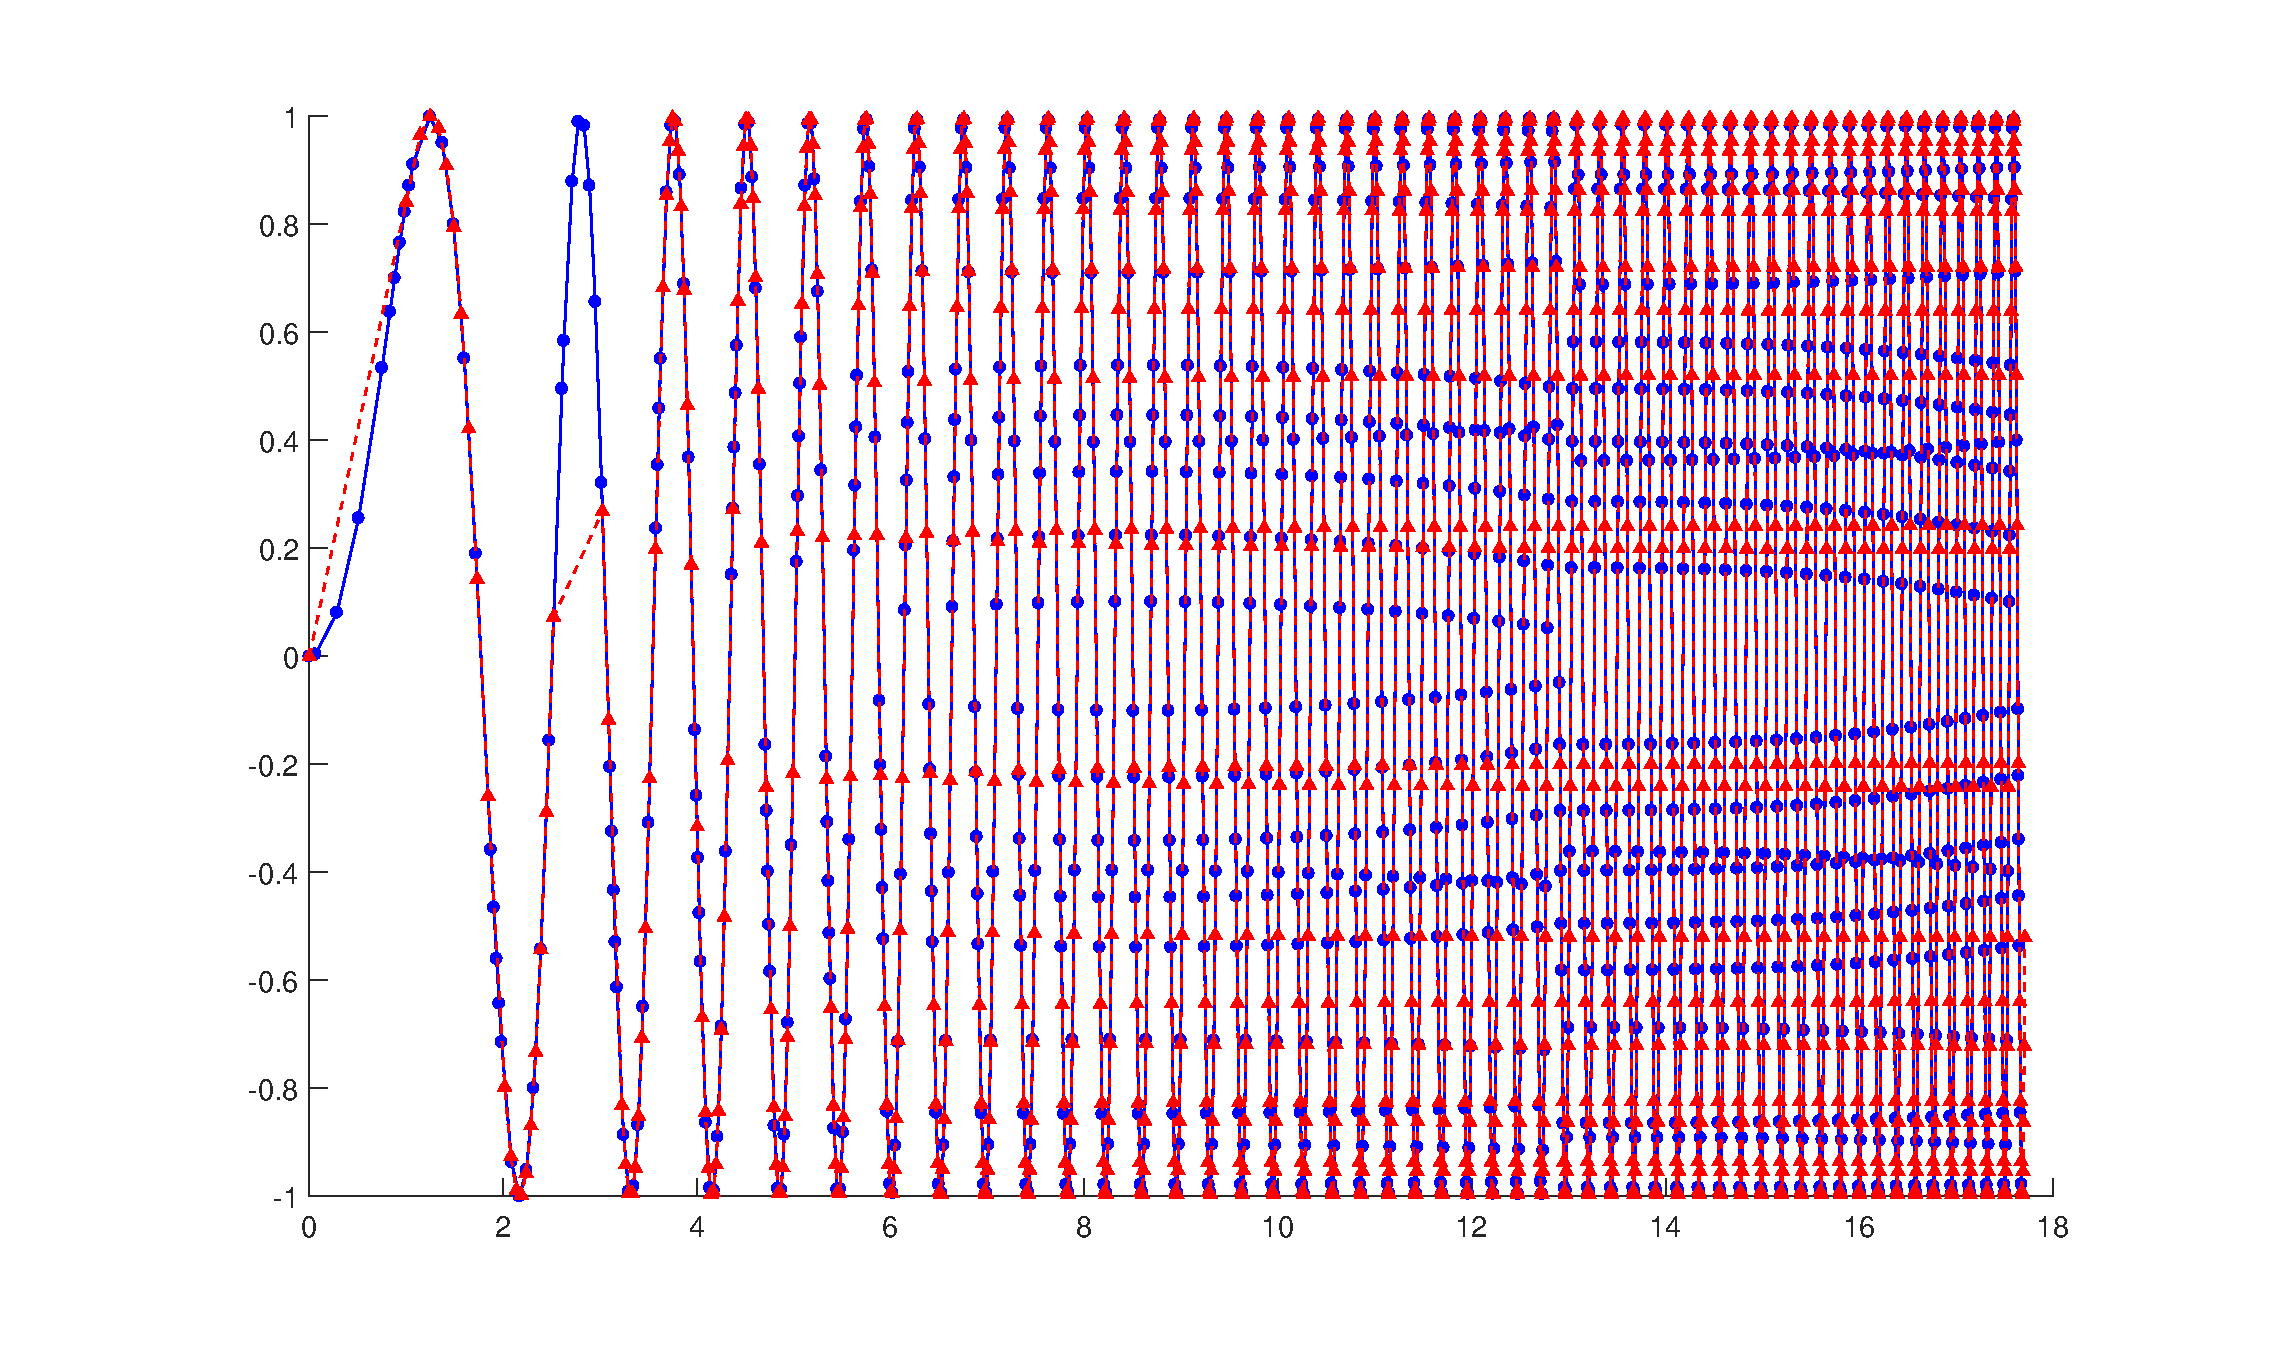
\includegraphics[trim = 41mm 0mm 30mm 0mm, clip, width=\linewidth]{plots/adapt/br}
	\caption{Vergleich der Strategie aus Kapitel \ref{chap:5.1.1} mit $c=6 \cdot10^{-3}$ (rot, 1087 Schritte) mit der gemischten Strategie mit $c=1.3 \cdot10^{-2}$ (blau, 1097 Schritte) }
	\label{fig:br}
	
\end{figure}

\begin{figure}[H]
	\centering
	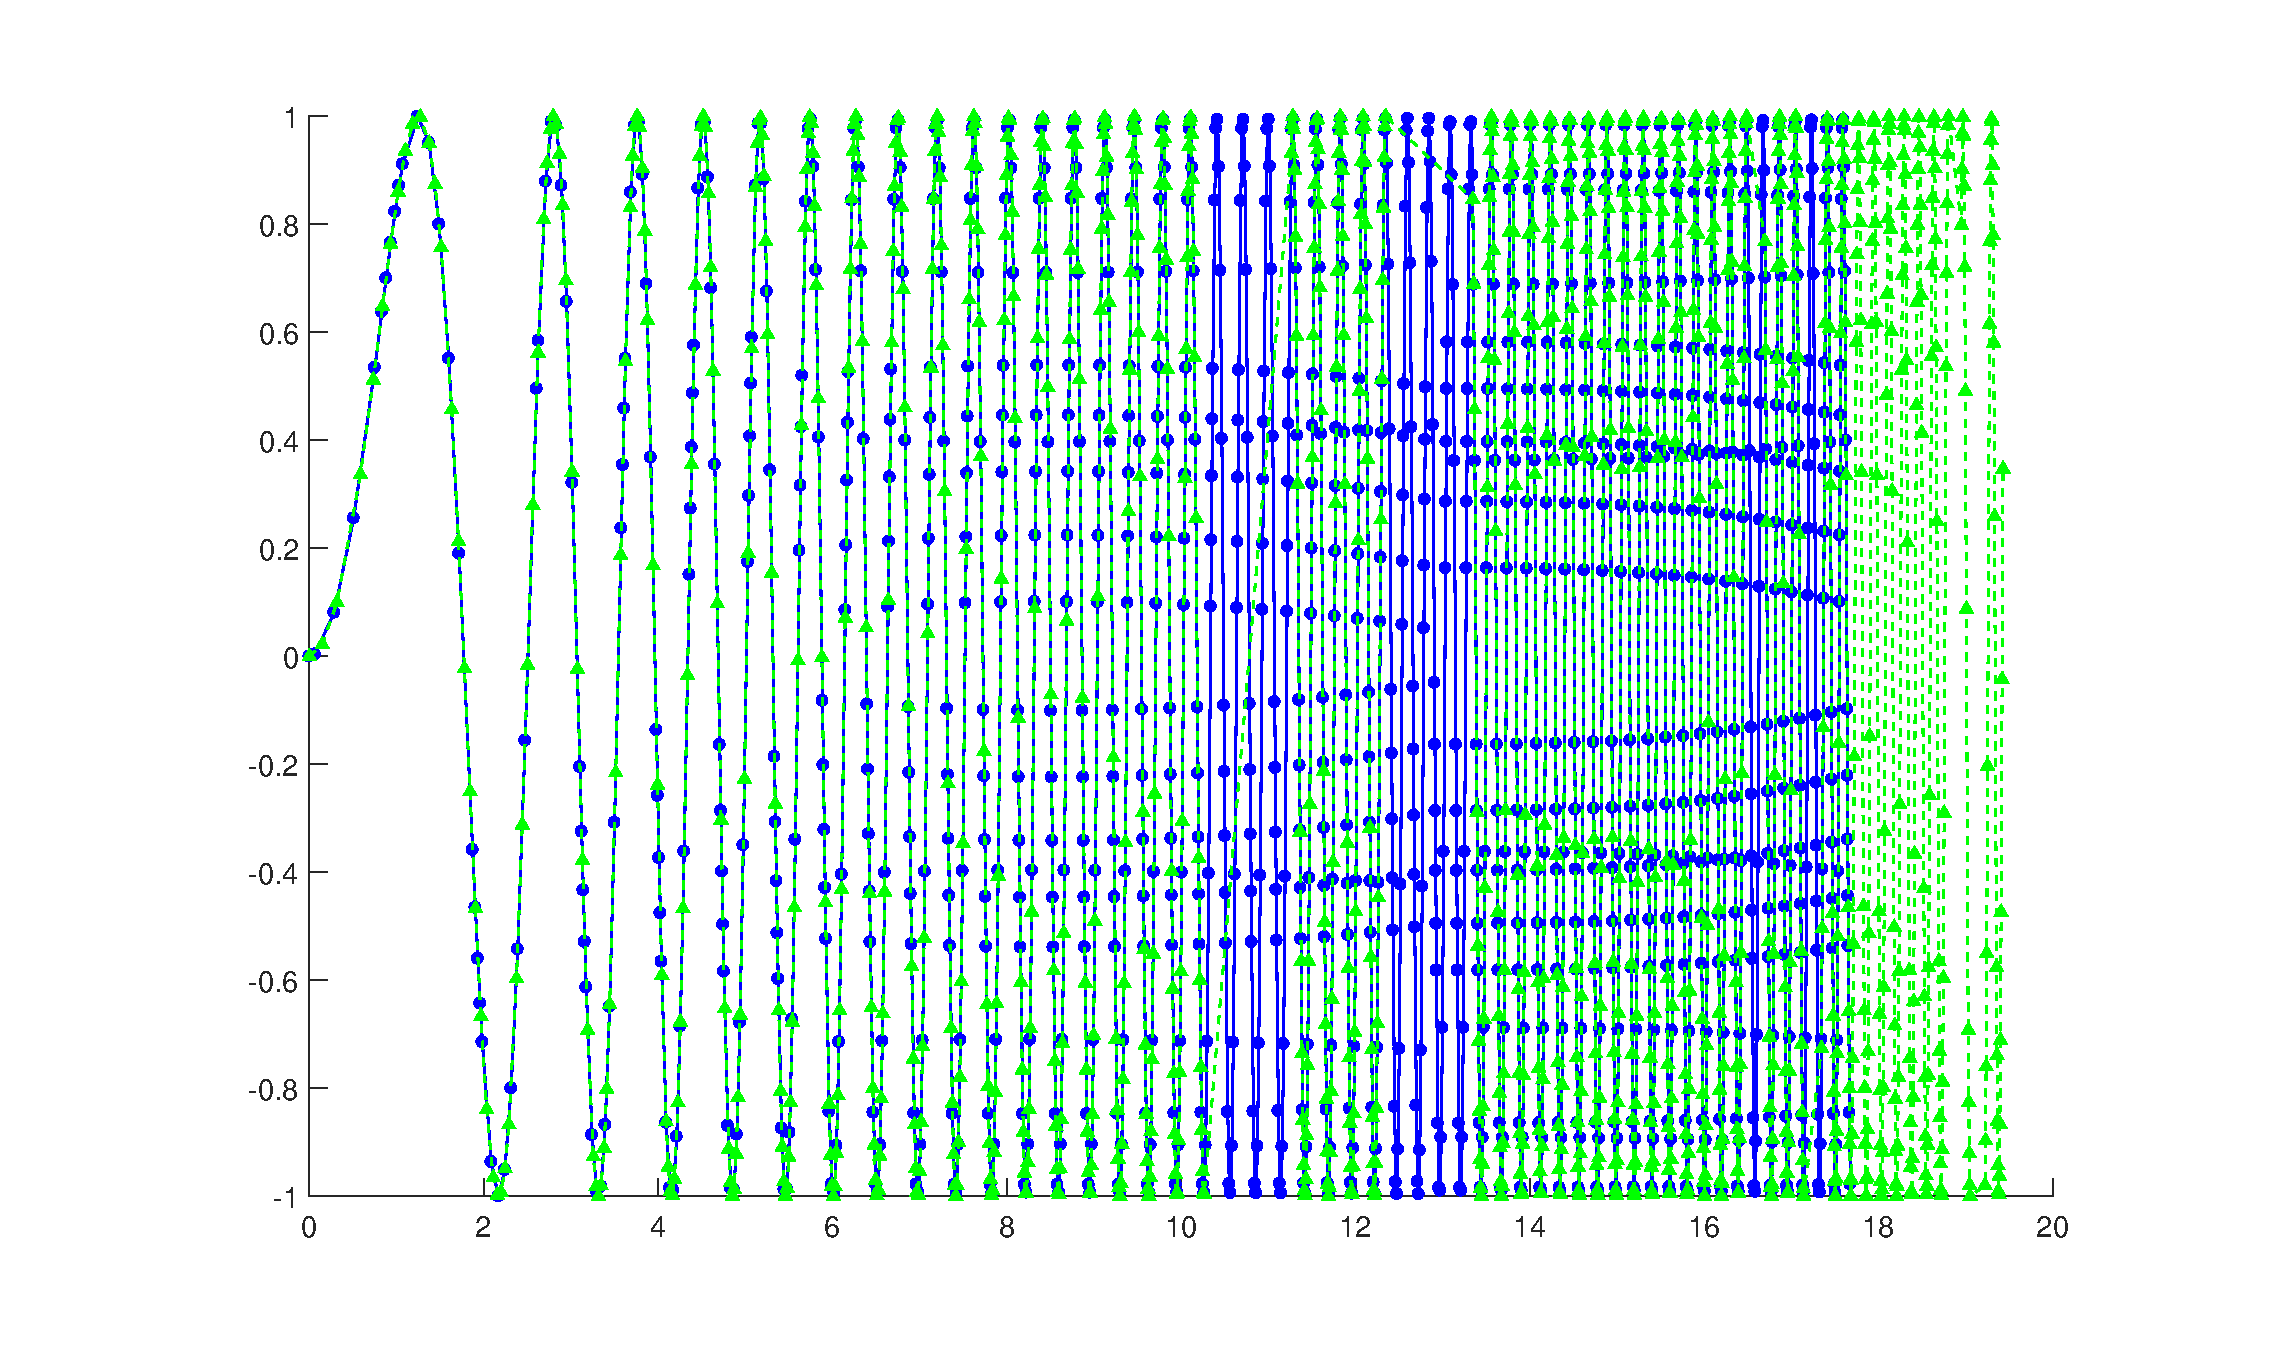
\includegraphics[trim = 41mm 0mm 30mm 0mm, clip, width=\linewidth]{plots/adapt/bg}
	\caption{Vergleich der Strategie aus Kapitel \ref{chap:5.1.3} mit $c=7.4\cdot10^{-2}$ (grün, 1074 Schritte) mit der gemischten Strategie mit $c=1.3 \cdot10^{-2}$ (blau, 1097 Schritte) }
	\label{fig:bg}
\end{figure}

\section{Implementierung von Niveaulinien}
\subsection{Problemstellung und Idee der Implementierung}

Die bisherigen Algorithmen finden Paare $(x_i,y_i)_{i=1,\dots N}$, sodass für $F(x_i,y_i)=0$ für $i=1,\dots, N$ und stellen damit die Nullstellenmenge von $F$ (oder nur einen Teil davon) näherungsweise graphisch dar. 

Im Folgenden sind $c_1,\dots, c_k \in \R$ gegeben und es sollen für $j=1,\dots,k$ die Teilmengen von $\{ (x,y) \in \R^2 : F(x,y)=c_j \}$ graphisch dargestellt werden.

Grundsätzlich ist dieses Problem einfach auf die vorherigen Algorithmen zurückzuführen, indem man die Nullstellenmengen der Funktionen $F_j(x,y) := F(x,y) -c_j$ graphisch darstellt.

Bei den vorherigen Algorithmen musste ein Startwert $(x_0,y_0) \in \R^2$ übergeben werden, für den gilt $F(x_0,y_0)=0$, also müsste in diesem Fall $k$ Startwerte $(x_j,y_j) \in \R^2$ übergeben werden, sodass
\[
F(x_j,y_j) = c_j \qquad j=1,\dots k.
\]

Dies stellt sich in der Praxis als sehr benutzerunfreundlich heraus, da die Gleichungen $F(x_j,y_j)=c_j$ im Allgemeinen nicht einfach zu lösen sind. 

Aus diesem Grund wurde ein Algorithmus implementiert, der in einem gegebenen Intervall $[a,b]\times[c,d] \subset \R^2$ entsprechende $(x_j,y_j)$ sucht und anschließend für $j=1,\dots, k$ einen der vorherigen Algorithmen mit der Funktion $F_j$ und den Startwerten $(x_j,y_j)$ aufruft. 

Der wesentliche Schritt ist also, nach Möglichkeit Nullstellen von $F_j$ in $[a,b] \times [c,d]$ zu finden. Das Newton-Verfahren im $\R^n$ steht hier nicht zur Verfügung, da nur es für Funktionen $G: \R^n \to \R^n$ anwendbar ist. Wegen der Regularitätsforderung  an die Jacobi-Matrix von $G$, ist es auch nicht möglich etwa $G(x,y) : = \binom{F(x,y)}{0}$ oder $G(x,y) : = \binom{F(x,y)}{F(x,y)}$ zu setzen und damit das Newton-Verfahren zu verwenden.

Es wird daher folgende Strategie verwendet:
\begin{itemize}
	\item Sei $m:= \binom{m_x}{m_y} := \binom{(a+b)/2}{(c+d)/2}$. Berechne $F(m)$. Falls $F(m)=0$ sind wir fertig, falls $F(m)<0$ betrachte $-F$. Wir können also im folgenden annehmen $F(m)>0$.
	\item Werte mithilfe geeigneter Schleifen $F$ an verschiedenen $(x,y) \in [a,b]\times [c,d]$ aus, bis $(x,y)$ mit $F(x,y)\le 0$ gefunden wird. Tritt dies nicht ein, bricht der Algorithmus an der Stelle ohne Ergebnis ab. Ist $F(x,y)=0$ sind wir fertig. Wir können also im Folgenden annehmen, dass $F(x,y)<0$ ist.
	\item Sei nun $\Psi : [0,1] \to \R^2 : t \mapsto \binom{m_x}{m_y} + t \binom{x-m_x}{y-m_y}$. Dann ist $ G:= \Psi \circ F : [0,1] \to \R$ stetig mit $G(0)>0$ und $G(1)<0$. Mithilfe des Bisektionsverfahrens kann man eine Nullstelle $t_0$ von $G$ finden.
	\item Dann ist $\Psi(t_0) \in [a,b] \times [c,d]$ eine Nullstelle von $F$.
\end{itemize} 
Diese Strategie hat in unseren Tests immer die Nullstellen gefunden. Nullstellen die gleichzeitig Extremstellen der Funktion $F$ sind, können damit nur durch großen Zufall gefunden werden, da die Funktion bei ihnen keinen Vorzeichenwechsel macht. Das ist kein großer Mangel, da diese Nullstellen aber unterinteressant sind, denn dort ist $\diff{F}{x}=0$ und $\diff{F}{y}=0$, was sie als Startwerte eher unbrauchbar macht.

\subsection{Details der Implementierung}

Es wurde also eine Funktionen der Art
\begin{verbatim}
nivlines (F, dFx, dFy, Z, A, B, C, D, Steps, StepWidth)
\end{verbatim}
%hier müsste normal stehen was F dFx dFy sind, das wird aber wohl schon oft genung gestanden sein
implementiert. Dabei sind:
\begin{itemize}
	\item \verb|Z| ein Vektor ist, der die Funktionswerte enthält, zu denen Niveaulinien geplottet werden sollen. Bezeichne $k$ im Folgenden die Länge von \verb|Z|).
	\item \verb|A|, \verb|B|, \verb|C|, \verb|D| jeweils Vektoren der Länge $k$, sodass ein Startwert für die Niveaulinie zu \verb|Z(j)| im Intervall [\verb|A(j)|, \verb|B(j)|]$\times$[ \verb|C(j)|, \verb|D(j)|] gesucht wird. Alternativ können auch Skalare übergeben werden, die wie Vektoren mit konstanten Einträgen behandelt werden.
	\item  \verb|Steps| und \verb|StepWidth| sind ebenfalls Vektoren der Länge $k$ oder Skalare, die die Schrittanzahl bzw. Schrittweite übergeben.
\end{itemize}

Die Implementierung der Funktion sieht dann im Wesentlichen (Assertions etc. wurden im Listing weggelassen) so aus:

\lstinputlisting[firstline=1, lastline=1000,caption=Ich bin ein Beispiel-Lisitng]{code/nivlines4.m}

%das sind jetzt sehr informatik / matlab-syntax-lastige dinge, die man auch streichen kann
%aber falls man den code wo einbindet sollte man es vlt erwähnt haben, damit die leute nicht über unbekannte syntax stolpern

Da die Anzahl der Datenpunkte für unterschiedliche Niveaulinien sehr unterschiedlich sein kann (zB wegen unterschiedlicher Länge oder Krümmung) und man die jeweiligen Anzahl je nach Algorithmus im Vorhinein auch nicht weiß, ist es nicht sinnvoll, alle Vektoren der $x$- bzw. $y$-Werte der Punkte für die einzelnen Niveau-Linien in gemeinsame Matrizen der Art $X, Y \in \R^{k \times maxSteps}$ zu schreiben.


der Punkte für die einzelnen Niveaulinien in Matrix $X \in \R^{k \times maxSteps}$ zu schreiben. Stattdessen bietet sich ein cell-Arays an, der $k$ Vektoren der Länge $Steps$ enthält. Der Zugriff auf die einzelnen Vektoren erfolgt durch \verb|X{j}|.

\subsection{Tests}
Sei %(x.^2+y.^2+10^-2).^-1 + ((x-0.5).^2+y.^2+10^-2).^-1
\[
F(x,y) := \frac{1}{x^2+y^2+10^{-2}} + \frac{1}{(x-0.5)^2+y^2+10^{-2}}
\]

Sei $Z:= (10,15,20,25,800/29,30,40,60,80,30,40,60,80)$ der Vektor der Funktionswerte, für die Niveau-Linien geplottet werden sollen. Für alle Werte wurden Startpunkte im Intervall $[0,1/4]\times[0,1]$ gesucht, für jene Werte, die im Vektor $Z$ doppelt vorkommen, wurde zusätzlich im Intervall $[1/2,3/4]\times[0,1]$ nach einem Startwert gesucht. Die Motivation für die Auswahl des Wertes $800/29$ ist, dass $F(1/4,0)=800/29$ und $DF(1/4,0)=(0,0)$.

Die Schrittweite betrug $2\cdot 10^{-3}$ die Schrittanzahl 2000 für die ersten fünf Niveaulinien bzw. 500 für die Restlichen.

\begin{figure}[H]
	\centering
	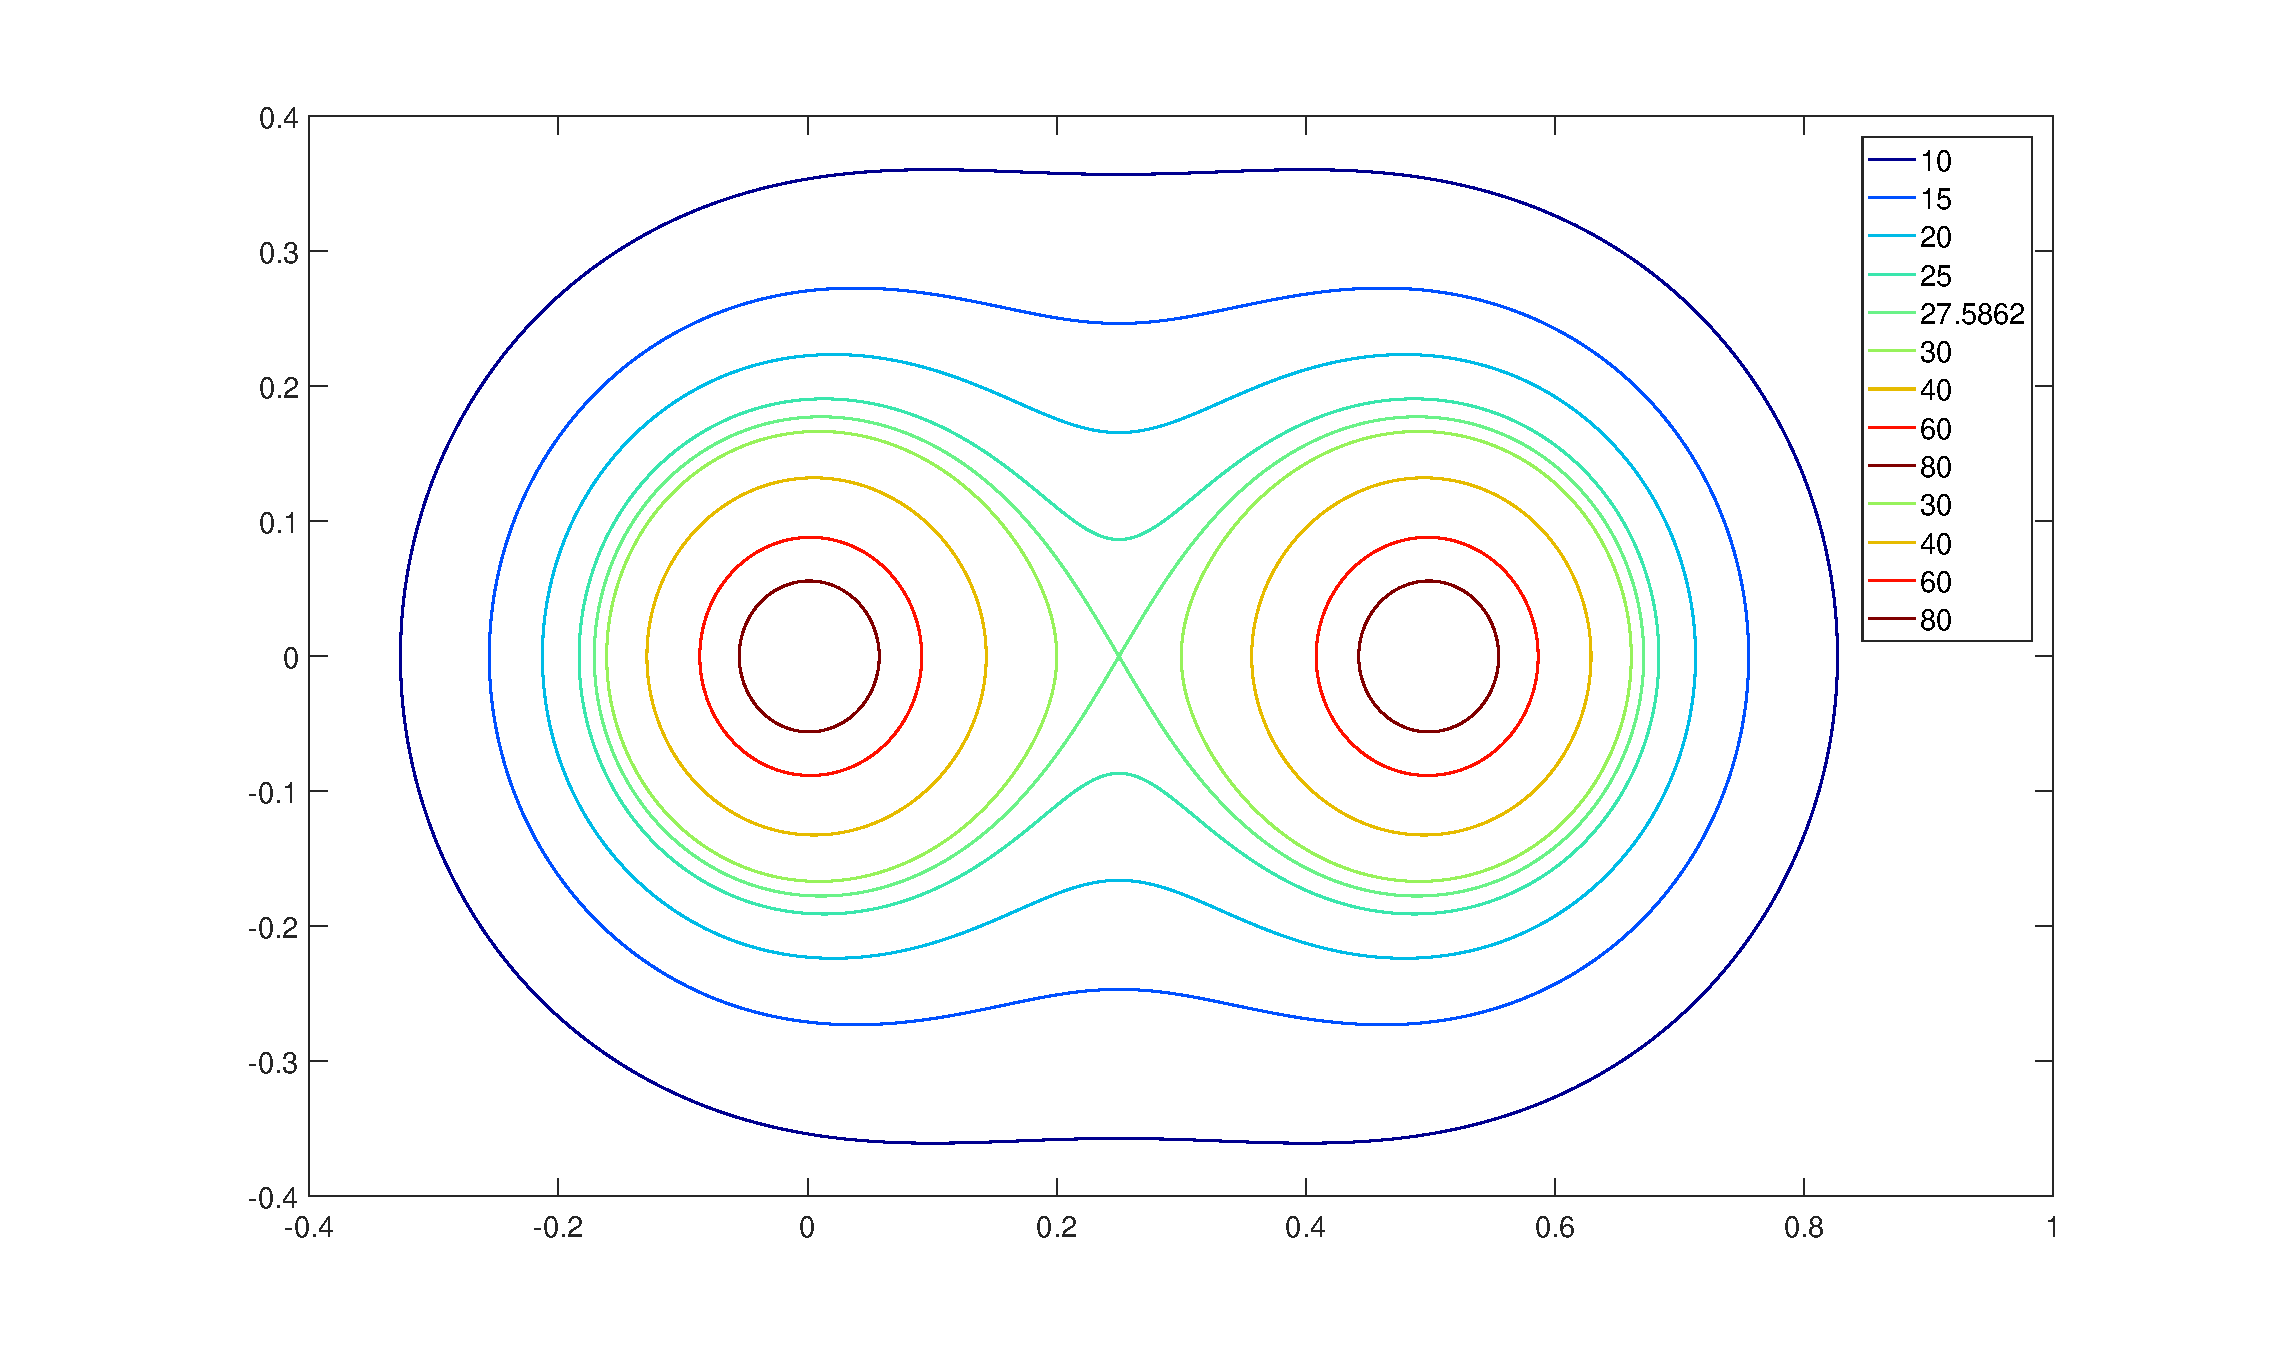
\includegraphics[trim = 41mm 0mm 35mm 0mm, clip, width=\linewidth]{plots/niveau/test5_}

\end{figure}

\section{Anhang: Code-Listings}
\lstinputlisting[firstline=1, lastline=1000,caption=Implementierung der Nullstellensuche im $\R^2$]{code/findZero.m}
%man wird wohl nur einzelne Ausschnitte im Fließtext haben wollen





\end{document}
